\chapter{Random Forests}
\label{ch:random_forests}

\begin{wrapfigure}{o}{0.85\textwidth}
    \vspace{-0.5cm}
    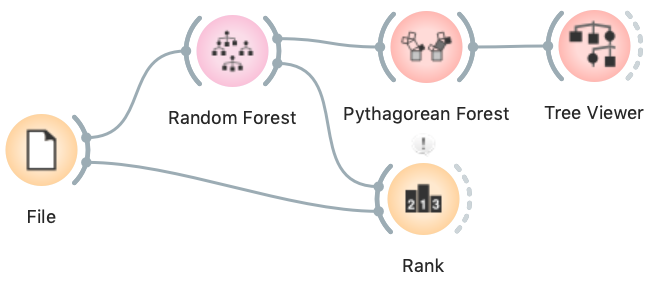
\includegraphics[scale=0.4]{workflow.png}
\end{wrapfigure}

Random forests, a modeling technique introduced in 2001, is still one of the best performing classification and regression techniques. Instead of building a tree by always choosing the a feature that seems to separate best at that time, it builds many trees in slightly random ways. Therefore the induced trees are different. For the final prediction the trees vote for the best class.

\begin{figure}[h]
    \centering
    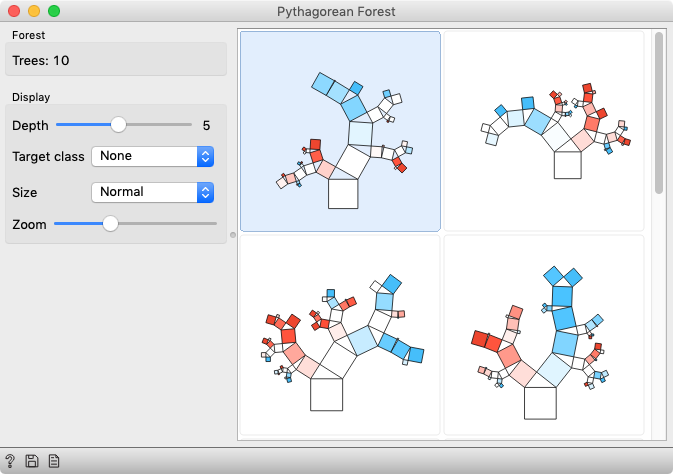
\includegraphics[scale=0.35]{pythagorean.png}
    \caption{The \widget{Pythagorean Forest} widget shows us how random the trees are. If we select a tree, we can observe it in a \widget{Tree Viewer}.}
\end{figure}

There are two sources of randomness: (1) training data is sampled with replacement, and (2) the best feature for a split is chosen among a subset of randomly chosen features.

Which features are the most important? The creators of random forests also defined a procedure for computing feature importances from random forests. In Orange, you can use it with the Rank widget.

\begin{figure}[h]
    \centering
    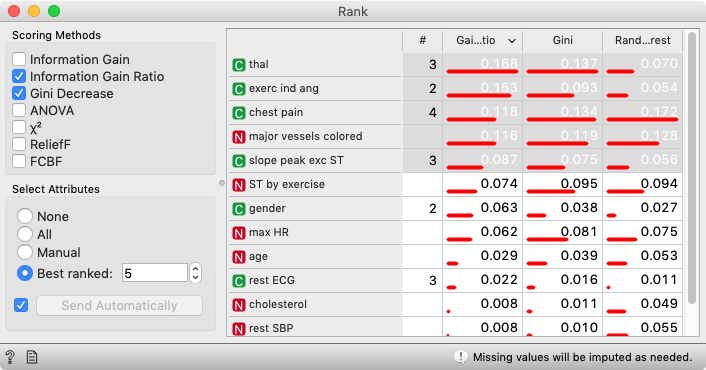
\includegraphics[scale=0.35]{rank.png}
    \caption{Feature importance according to two univariate measures (gain ratio and gini index) and random forests. Random forests also consider combinations of features when evaluating their importance. }
\end{figure}
